
\definecolor{cd9d9d9}{RGB}{217,217,217}
\definecolor{c888888}{RGB}{136,136,136}
\definecolor{cc8c8c8}{RGB}{200,200,200}

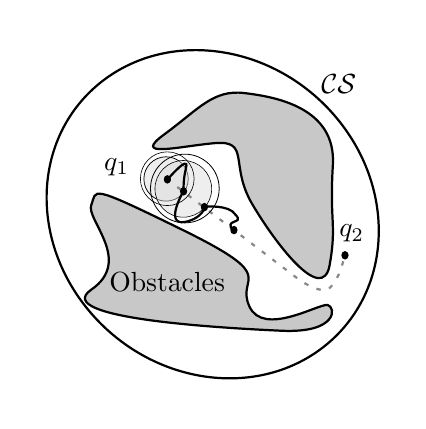
\begin{tikzpicture}[y=0.65pt, x=0.65pt,yscale=-1, inner sep=0pt, outer sep=0pt]
  \begin{scope}% layer1
    % path4348-7-9
    \path[cm={{0.88069687,0.0,0.0,0.88069687,(30.925926,8.8427197)}},draw=black,fill=cd9d9d9,miter
      limit=4.00,fill opacity=0.450,line width=0.273pt]
    (347.2399,152.3163)arc(0:180:14)arc(-180:0:14) --
    cycle;

    % path4348-7-9-7
    \path[cm={{1.1259005,0.0,0.0,1.1259005,(-41.191,-23.012876)}},draw=black,fill=cd9d9d9,miter
      limit=4.00,fill opacity=0.450,line width=0.213pt]
    (347.2399,152.3163)arc(0:180:14)arc(-180:0:14) --
    cycle;

    % path5244
    \path[draw=c888888,dash pattern=on 1.60pt off 3.20pt,line join=miter,line
      cap=butt,miter limit=4.00,line width=0.800pt] (324.7640,142.9724) .. controls
    (324.7640,142.9724) and (392.3443,194.3298) .. (397.6213,198.4045) .. controls
    (402.3196,202.0323) and (410.6305,205.8633) .. (413.9100,204.5917) .. controls
    (416.8177,203.4642) and (420.7090,195.9224) .. (421.4862,193.4800) .. controls
    (422.4768,190.3665) and (423.7590,185.6513) .. (423.7590,185.6513);

    % path2160
    \path[cm={{0.51754158,0.59470899,-0.78330399,0.64302546,(277.06748,-164.97712)}},draw=black,line
      join=miter,line cap=butt,line width=0.800pt]
    (502.2720,157.7193)arc(0:180:122 and
    86)arc(-180:0:122 and 86) -- cycle;

    % path3136
    \path[draw=black,fill=cc8c8c8,line join=miter,line cap=butt,even odd rule,line
      width=0.800pt] (323.5714,118.0765) .. controls (342.3822,104.3382) and
    (350.5113,93.1397) .. (367.8571,95.2193) .. controls (385.2029,97.2990) and
    (419.0623,103.2255) .. (417.1429,135.2193) .. controls (415.2234,167.2132) and
    (419.3643,167.7282) .. (415.3825,190.6736) .. controls (411.4008,213.6191) and
    (384.7193,178.1899) .. (372.1429,156.6479) .. controls (359.5665,135.1059) and
    (371.4345,121.3381) .. (351.4286,123.0765) .. controls (331.4227,124.8148) and
    (304.7606,131.8148) .. (323.5714,118.0765) -- cycle;

    % path3138
    \path[draw=black,fill=cc8c8c8,line join=miter,line cap=butt,even odd rule,line
      width=0.800pt] (282.8571,157.3622) .. controls (286.1376,149.2915) and
    (279.6176,144.7773) .. (334.2857,171.6479) .. controls (388.9538,198.5185) and
    (362.8864,196.4968) .. (370.7143,213.7908) .. controls (378.5422,231.0847) and
    (409.6606,211.9285) .. (414.2857,213.0765) .. controls (418.9109,214.2244) and
    (419.9284,228.7908) .. (388.5714,227.3622) .. controls (357.2145,225.9336) and
    (259.4398,220.6704) .. (282.8571,204.5050) .. controls (306.2745,188.3397) and
    (279.5767,165.4328) .. (282.8571,157.3622) -- cycle;

    % path3146
    \path[cm={{0.4204395,0.0,0.0,0.4204395,(301.97396,131.87051)}},draw=black,fill=black]
    (293.9544,127.3150)arc(-0:180:4 and
    4.798)arc(-180:0:4 and 4.798) -- cycle;

    % path3144-4
    \path[cm={{0.4204395,0.0,0.0,0.4204395,(203.23155,89.696643)}},draw=black,fill=black]
    (293.9544,127.3150)arc(-0:180:4 and
    4.798)arc(-180:0:4 and 4.798) -- cycle;

    % path4348-7
    \path[cm={{1.066689,0.0,0.0,1.066689,(-30.387755,-19.628005)}},draw=black,miter
      limit=4.00,line width=0.225pt]
    (347.2399,152.3163)arc(0:180:14)arc(-180:0:14) --
    cycle;

    % path3144-4-0
    \path[cm={{0.4204395,0.0,0.0,0.4204395,(212.23282,96.333932)}},draw=black,fill=black]
    (293.9544,127.3150)arc(-0:180:4 and
    4.798)arc(-180:0:4 and 4.798) -- cycle;

    % path4462
    \path[draw=black,line join=miter,line cap=butt,line width=0.800pt]
    (325.0000,143.5229) .. controls (325.0000,143.5229) and (337.3919,129.0073) ..
    (335.5357,136.6479) .. controls (333.5526,144.8109) and (334.2857,150.1300) ..
    (334.2857,150.1300);

    % path4348-7-7
    \path[cm={{1.3636764,0.0,0.0,1.3636764,(-119.57563,-59.410424)}},draw=black,miter
      limit=4.00,line width=0.293pt]
    (347.2399,152.3163)arc(0:180:14)arc(-180:0:14) --
    cycle;

    % path3144-4-0-5
    \path[cm={{0.4204395,0.0,0.0,0.4204395,(223.84497,105.10147)}},draw=black,fill=black]
    (293.9544,127.3150)arc(-0:180:4 and
    4.798)arc(-180:0:4 and 4.798) -- cycle;

    % path4511
    \path[draw=black,line join=miter,line cap=butt,line width=0.800pt]
    (333.9817,149.9171) .. controls (333.9817,149.9171) and (321.6451,171.4668) ..
    (337.5172,166.2059) .. controls (344.1210,164.0170) and (345.7247,159.3873) ..
    (345.7247,159.3873) -- (345.7247,159.3873);

    % path4513
    \path[draw=black,line join=miter,line cap=butt,line width=0.800pt]
    (345.7143,158.4336) .. controls (345.7143,158.4336) and (359.6429,157.0050) ..
    (363.0357,162.8979) .. controls (368.5714,168.4336) and (355.4744,164.7300) ..
    (362.0816,172.0514);

    % path3144-4-0-5-7
    \path[cm={{0.4204395,0.0,0.0,0.4204395,(240.22838,117.85464)}},draw=black,fill=black]
    (293.9544,127.3150)arc(-0:180:4 and
    4.798)arc(-180:0:4 and 4.798) -- cycle;

    % text3039
    \path[fill=black] (420.71426,173.43362) node[right] (text3039) {$q_2$};

    % text3043
    \path[fill=black] (290,141.29077) node[above right] (text3043) {$q_1$};

    % text3142
    \path[fill=black] (410.71429,90) node[right] (text3142) {$\mathcal{CS}$};

    \node (obst) at  (325,200) {Obstacles};

  \end{scope}

\end{tikzpicture}
